
%(BEGIN_QUESTION)
% Copyright 2010, Tony R. Kuphaldt, released under the Creative Commons Attribution License (v 1.0)
% This means you may do almost anything with this work of mine, so long as you give me proper credit

This motor control circuit commands three motors to start and stop together:

$$\includegraphics[width=15.5cm]{i02399x01.eps}$$

Examine the control circuit and then explain how starting one motor starts up the others.  Also, determine what will happen if motor \#3 suffers an overload (i.e. OL3 warms up enough to trip).

\vskip 20pt \vbox{\hrule \hbox{\strut \vrule{} {\bf Suggestions for Socratic discussion} \vrule} \hrule}

\begin{itemize}
\item{} Explain why {\it inrush current} could be a problem in this three-motor control system, and identify at least one practical solution for it.
\item{} If motor \#2 were to become overloaded, would the system react any differently from an overloaded motor \#3?
\end{itemize}

\underbar{file i02399}
%(END_QUESTION)





%(BEGIN_ANSWER)

These three motors are all interlocked so that each one depends on the other.  If any of them them trips, all three shut off!

In the specific case of motor \#3, its tripping causes all three motors to shut off automatically.  However, motors \#1 and \#2 may still be ``jogged'' by pressing and holding the ``Start'' pushbutton.
 
%(END_ANSWER)





%(BEGIN_NOTES)


%INDEX% Final Control Elements, valve: electric actuator

%(END_NOTES)


